\documentclass{beamer}
\usetheme{Szeged}
\definecolor{beamer@andja}{rgb}{0.3, 0.6, 0.8}
\setbeamercolor{structure}{fg=beamer@andja}	
\usepackage{beamerthemeshadow}
\usepackage{url}
\usepackage[utf8]{inputenc}
\usepackage{graphicx}
\usepackage{color}
\usepackage{tikz}
\usepackage{caption}
\usepackage{subcaption}
\usepackage{dirtytalk}
\usepackage{amsthm}

\setbeamertemplate{footline}{\hspace*{.5cm}\scriptsize{\hspace*{50pt} \hfill\hspace*{.5cm}}\\
\vspace{20pt}}

\usepackage[english,serbian]{babel}

\begin{document}
\title{\Large Primena metoda mašinskog učenja za predviđanje potražnje automobilskih rezervnih delova \\ \vspace{5pt} \scriptsize {master rad}\\ \vspace{2pt}\small{mentor: dr Aleksandar Kartelj}}
\institute {\tiny{Matematički fakultet\\Univerzitet u Beogradu}}
\author{Anđelka Milovanović\\ \tiny 1033/2020}
\date{\tiny 27. septembar 2021.}

\setbeamertemplate{footline}
{
  \leavevmode
  \hbox{
  \begin{beamercolorbox}[wd=.49\paperwidth,ht=2.25ex,dp=1ex,center]{author in head/foot}
    \usebeamerfont{author in head/foot}{Anđelka Milovanović}
  \end{beamercolorbox}
  \begin{beamercolorbox}[wd=.49\paperwidth,ht=2.25ex,dp=1ex,center]{title in head/foot}
    \usebeamerfont{title in head/foot}{Master rad}
  \end{beamercolorbox}}
}


\begingroup
\setbeamertemplate{footline}{}
\begin{frame}
    \begin{tikzpicture}
        \node[anchor=north east, inner sep=2] (image) at (0,0)
        {
\includegraphics[width=1.8cm]{images/matf-light.png}};
        \node[anchor=north west, inner sep=2] (image) at (7,0)
        {
\includegraphics[width=1.3cm]{images/matf_logo.png}};
    \end{tikzpicture}
  \vspace{-0.53cm}
  \titlepage
\end{frame}
\endgroup

\setbeamertemplate{section in toc}[sections numbered]
\setbeamertemplate{subsection in toc}{\leavevmode\leftskip=3.2em\rlap{\hskip-2em\inserttocsectionnumber.\inserttocsubsectionnumber}\inserttocsubsection\par}
\setbeamerfont{subsection in toc}{size=\footnotesize}

\begin{frame}\frametitle{Sadržaj}\tableofcontents
\end{frame} 

\section{Uvod} 
\begin{frame} {Motivacija} 
\begin{itemize}
    \item Problem predviđanja potražnje (eng. \textit{demand forecasting}) je značajan i široko zastupljen problem u mnogim industrijama;
    \item Davanje najbolje procene potražnje za nekim proizvodom u budućnosti, pod zadatim ulaznim parametrima;
    \item Ušteda energije, ušteda materijala, smanjenje troškova, povećanje efikasnosti...
    \item Industrija popravki automobila: količine potrebnih rezervnih delova, isporuka delova, broj sati raspoloživih za popravku, broj dostupnih automehaničarskih radnji.
\end{itemize}

% \begin{figure}[!tbp]
%   \begin{subfigure}[b]{0.3\textwidth}
%     \includegraphics[width=\textwidth]{images/17_AM_FrankWagner.png}
%     \caption{\tiny{Frank O Wagner (radovi: 1986-2008)}} 
%     \label{fig:frank}
%   \end{subfigure}
%   \hspace{50pt}
%   \begin{subfigure}[b]{0.3\textwidth}
%     \includegraphics[width=\textwidth]{images/17_AM_AlexanderWolff.png}
%     \caption{\tiny {Alexander Wolff - Today Chair for Algorithms and Complexity, University of Würzburg}}
%     \label{fig:alexander}
%   \end{subfigure}
% %   \caption{\scriptsize{Google Scholar citiranja}}
% \end{figure}
\end{frame}

\begin{frame}{Opis problema}
\begin{enumerate}
    \item Problem kao vremenska serija:
    \begin{itemize}
        \item dnevno uzorkovanje promenljive koja predstavlja potražnju;
        \item fokus na predviđanju 1 korak unapred;
        \item predviđanje se temelji samo na prethodnim vrednostima posmatrane promenljive.
    \end{itemize}
    % Niz vrednosti promenljive koja predstavlja potražnju, merenih u uzastopnim i ekvidistantnim vremenskim trenucima (u ovom radu originalni uzorci su na dnevnom nivou). Cilj su predviđanja promenljive 1 korak unapred.
    \item Problem posmatran kroz atribute:
        \begin{itemize}
            \item regresioni problem koji zavisi od nekoliko atributa;
            \item rešavan je ansambl metodom ekstremnog gradijentnog pojačavanja (XGBoost).
        \end{itemize}
\end{enumerate}
\end{frame}

%%%%%%%%%%%%%%%%%%%%%%%%%%%%%%%%%%%%%%%%%%%%%%%%%%%%%
\section{Korišćene metode i metrike}
\subsection{Korišćene metode}
\begin{frame}{Korišćene metode}
\begin{itemize}
    \item Autoregresivni model pokretnih proseka za integrisane vremenske serije (ARIMA)
    
    \item Prophet\footnote{Razvijen je od strane Facebook zajednice.} (sezonalnost, praznici)
    \item XGBoost
\end{itemize}

\begin{figure}[!tbp]
  \begin{subfigure}[b]{0.4\textwidth}
    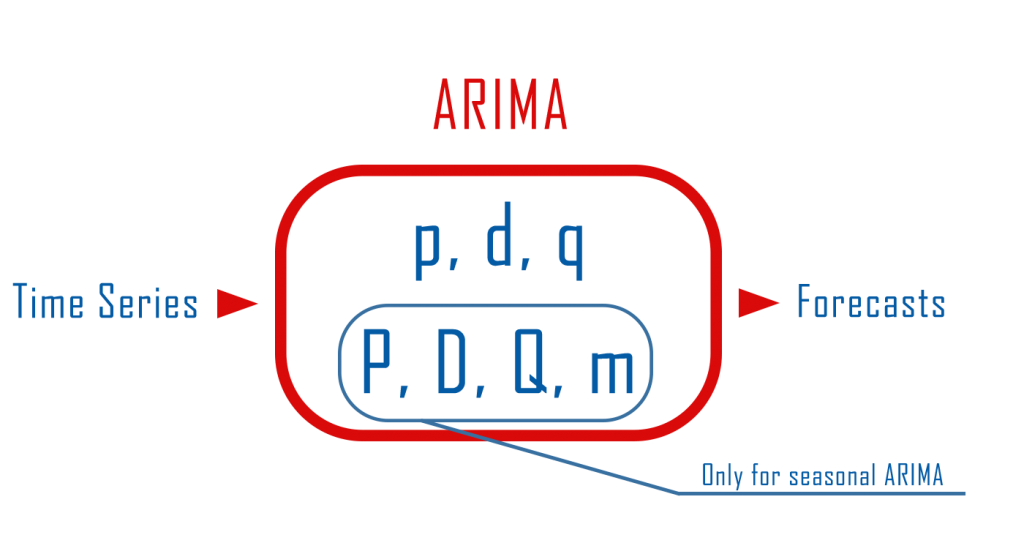
\includegraphics[width=\textwidth]{images/arima_schema.png}
    \caption{\tiny{Arima}} 
    \label{fig:arima}
  \end{subfigure}
  \hspace{50pt}
  \begin{subfigure}[b]{0.4\textwidth}
    
\includegraphics[width=\textwidth]{images/prophet_logo.png}
    \caption{\tiny {Prophet}}
    \label{fig:prophet}
  \end{subfigure}
%   \caption{\scriptsize{Google Scholar citiranja}}
\end{figure}

\end{frame}

\subsection{Metrike i kategorički atributi}
\begin{frame}{Metrike i kategorički atributi}
\begin{itemize}
    \item Standardne metrike i izmenjena SMAPE metrika 
    \begin{figure}
        \centering
        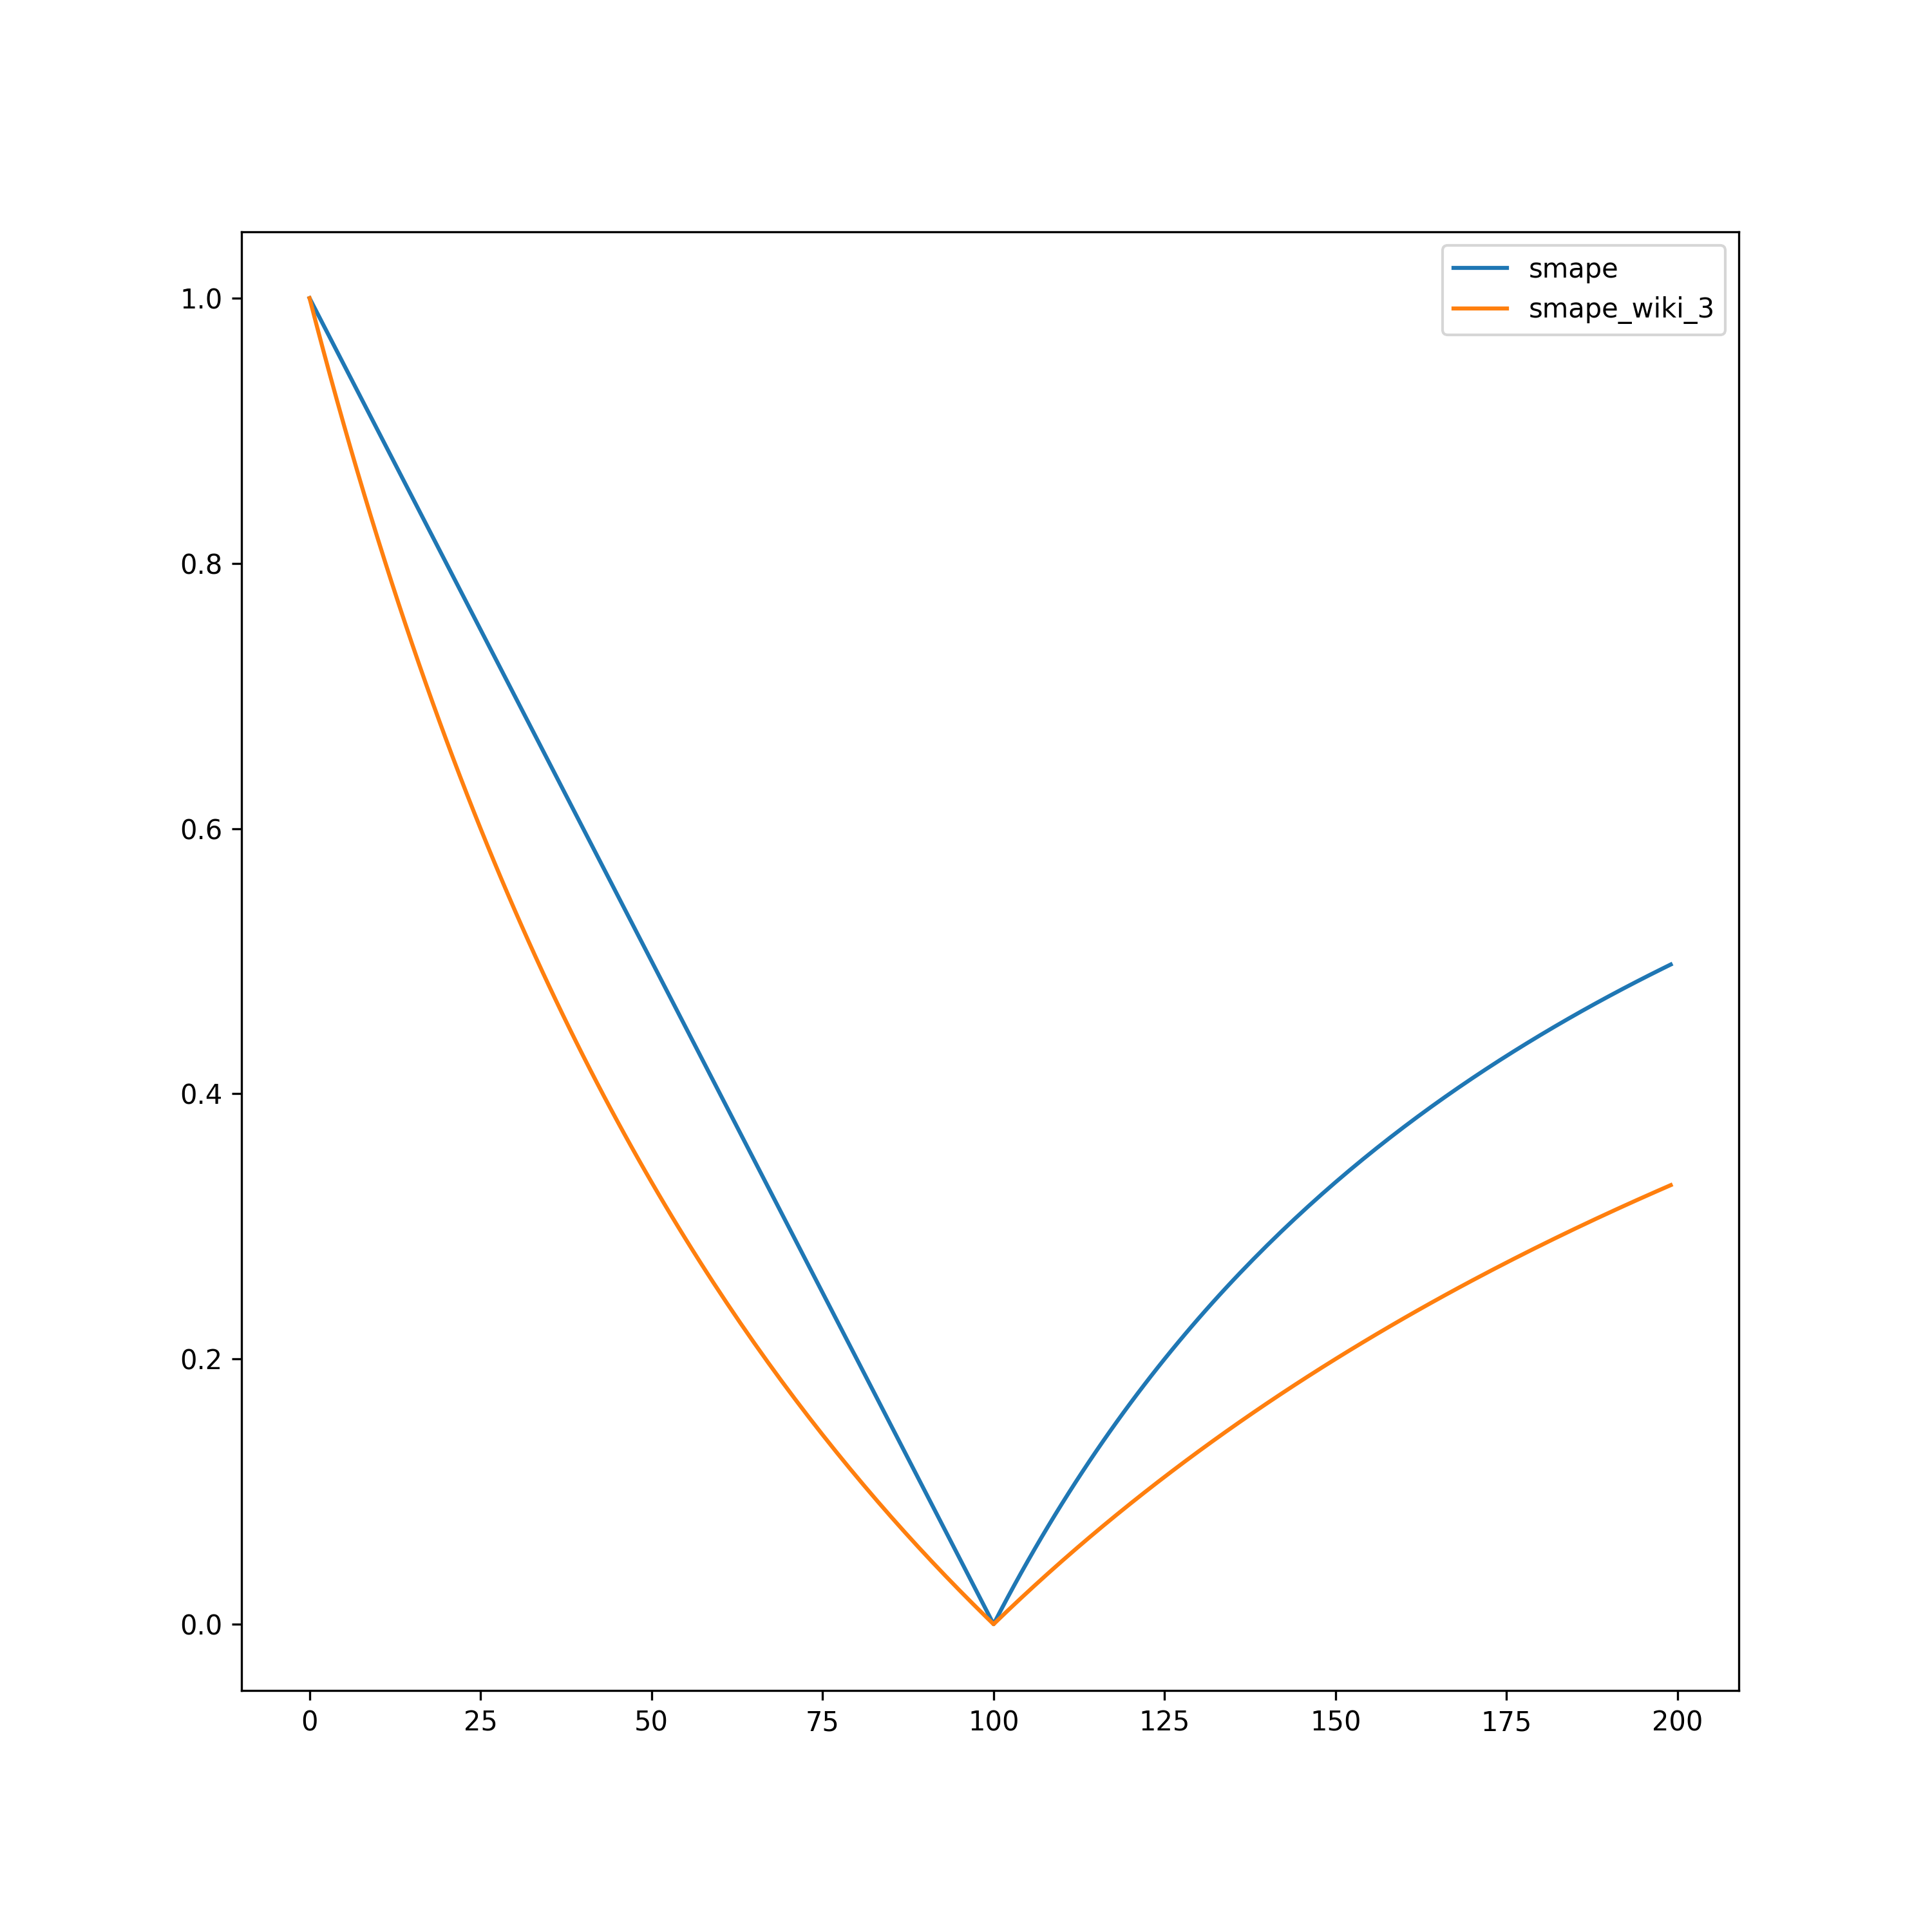
\includegraphics[width=0.4\textwidth]{images/smape_test.png}
        \vspace{-10px}
        \caption{Izmenjena SMAPE metrika (smape) i podrazumevana SMAPE metrika (smape\_wiki3)}
        \label{fig:smape_test}
    \end{figure}
    \vspace{-10px}
    \item Kodiranje uticajem (eng. \textit{Impact encoding})   
\end{itemize}
\end{frame}

\section{Podaci}
\begin{frame}{Podaci}
\begin{itemize}
    \item Švedska kompanija;
    \item Rezervisanje popravki automobila putem interneta (eng. \textit{booking portal});
    \item Početak rada krajem 2019. godine;
    \vspace{5px}
    \begin{figure}
        \centering
        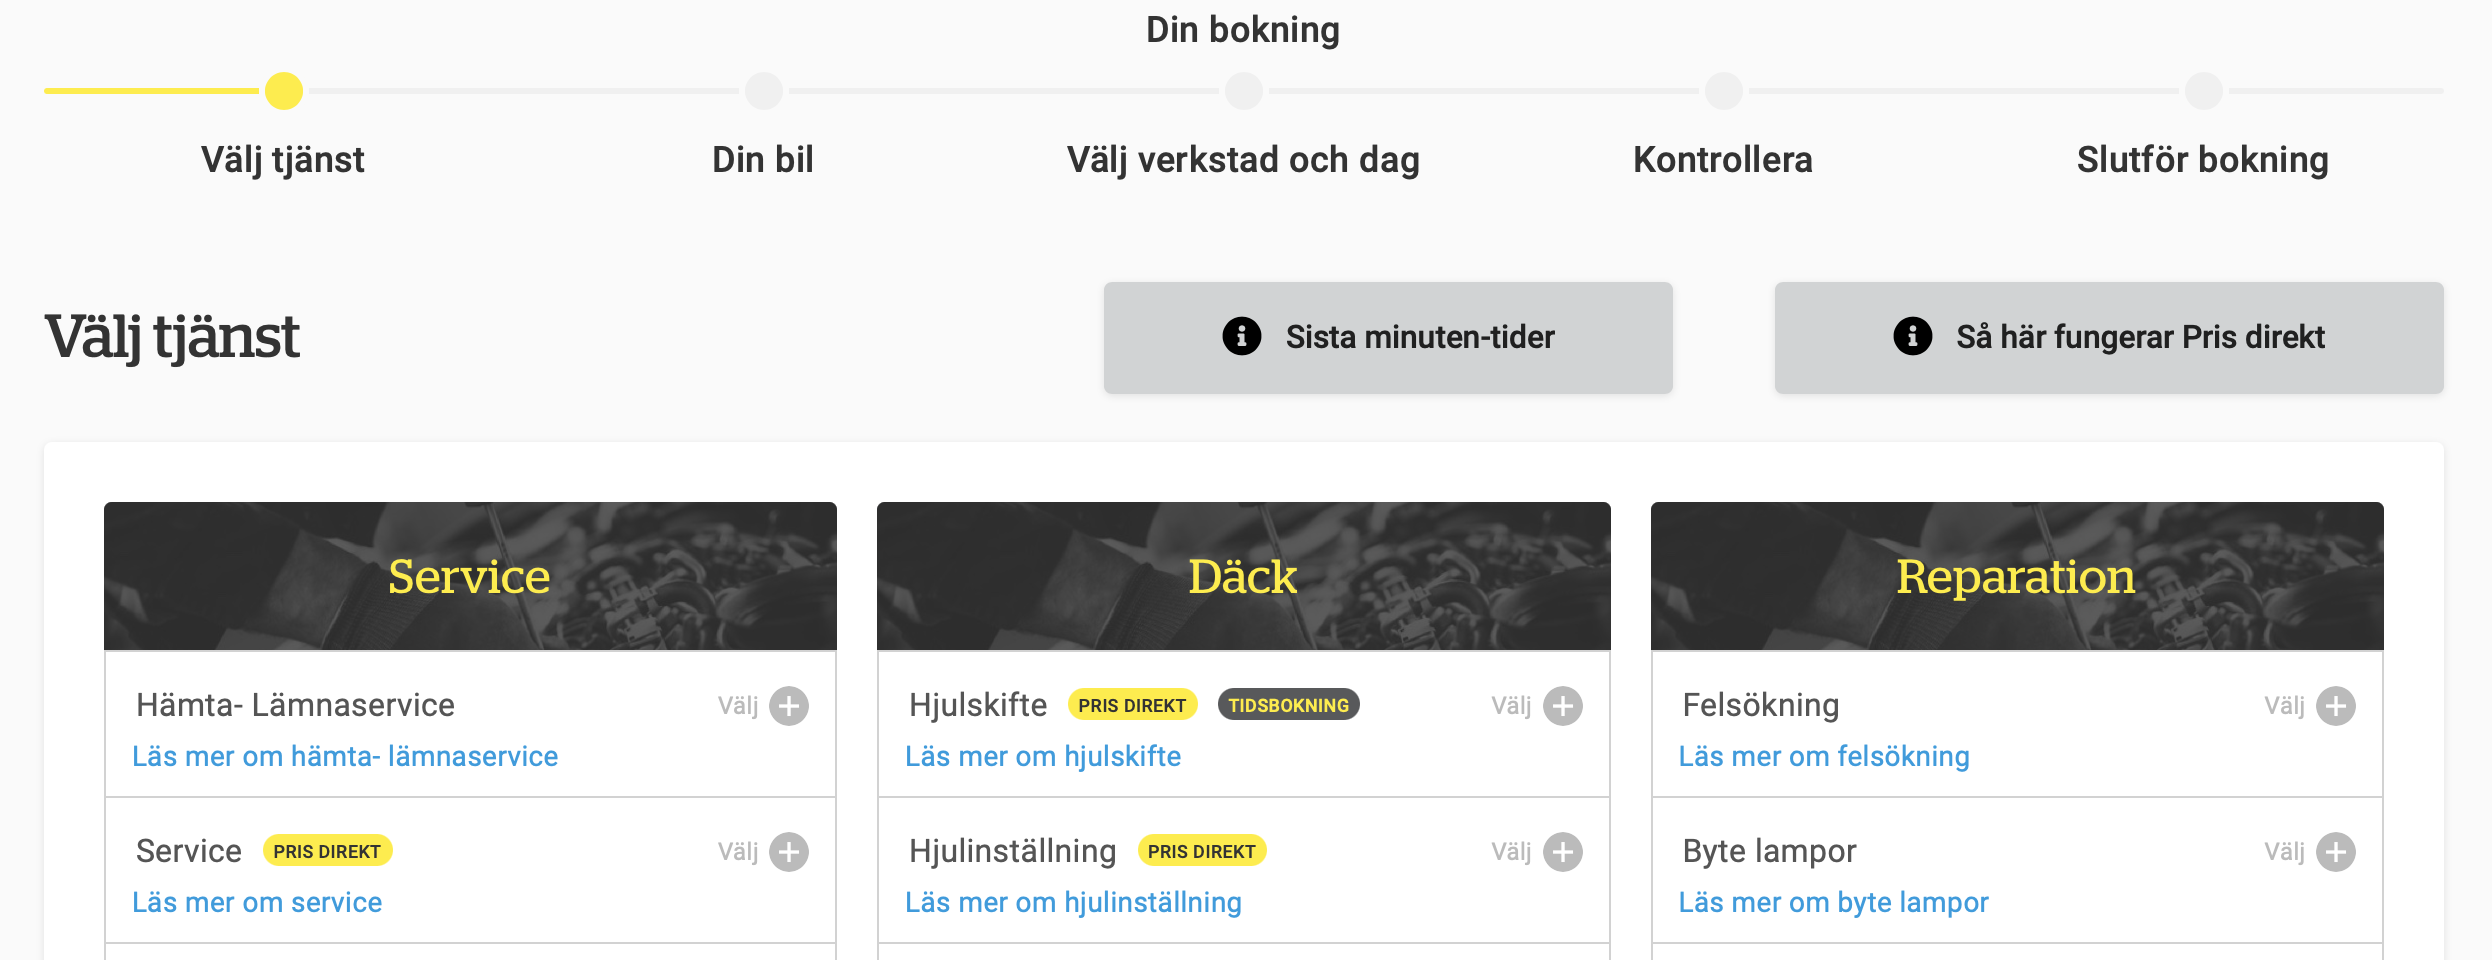
\includegraphics[width=0.8\textwidth]{images/swedish_company.png}
        \caption{Primer internet portala za rezervacije}
        \label{fig:booking_portal}
    \end{figure}
\end{itemize}
\end{frame}

\begin{frame}{Podaci}
    \begin{figure}
        \centering
        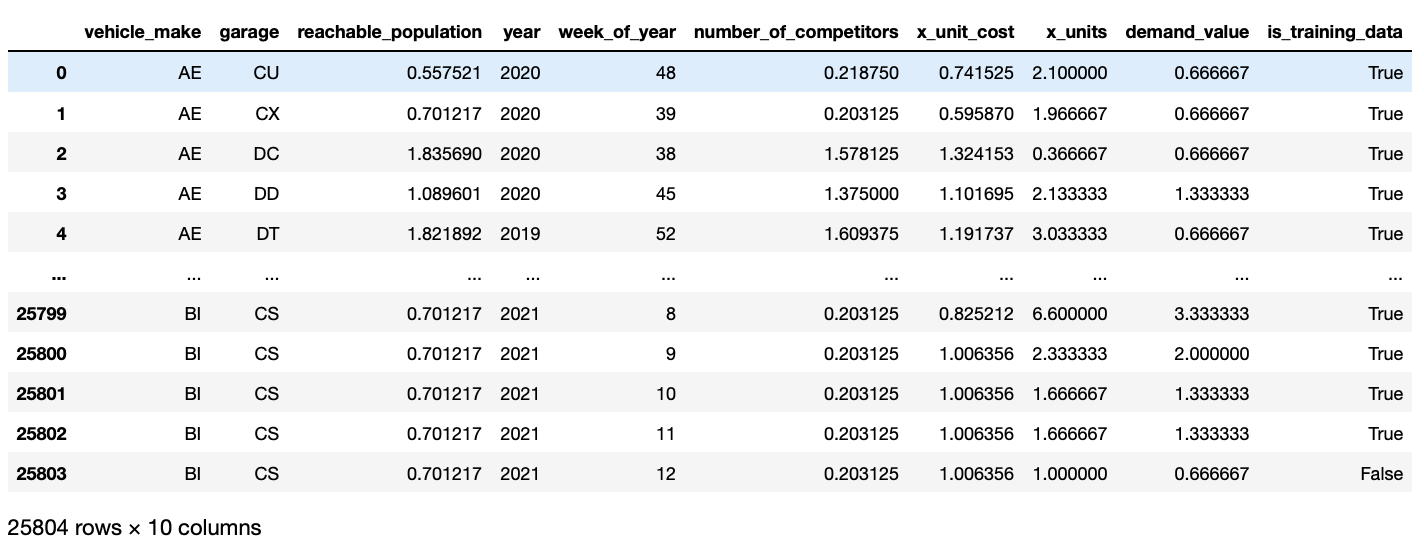
\includegraphics[width=1\textwidth]{images/grafici/atributi_primer.png}
        \caption{Primer skupa atributa i ciljne promenljive}
        \label{fig:primer_podataka}
    \end{figure}
\end{frame}

\begin{frame}{Obogaćivanje eksternim podacima}
\begin{itemize}
    \item Svaka automehaničarska radnja ima svoju geografsku širinu i geografsku dužinu;
    \item \textit{reachable\_population}: suma populacije velikih regiona u opsegu koji predstavlja rastojanje pređeno za 40 minuta vožnje, brzinom 60 km/h, od lokacije radnje;
    \item \textit{number\_of\_competitors}: broj drugih radnji u opsegu od 80km od automehaničarske radnje.
\end{itemize}
\end{frame}

\begin{frame}{Open Street Map}
\begin{figure}
    \centering
    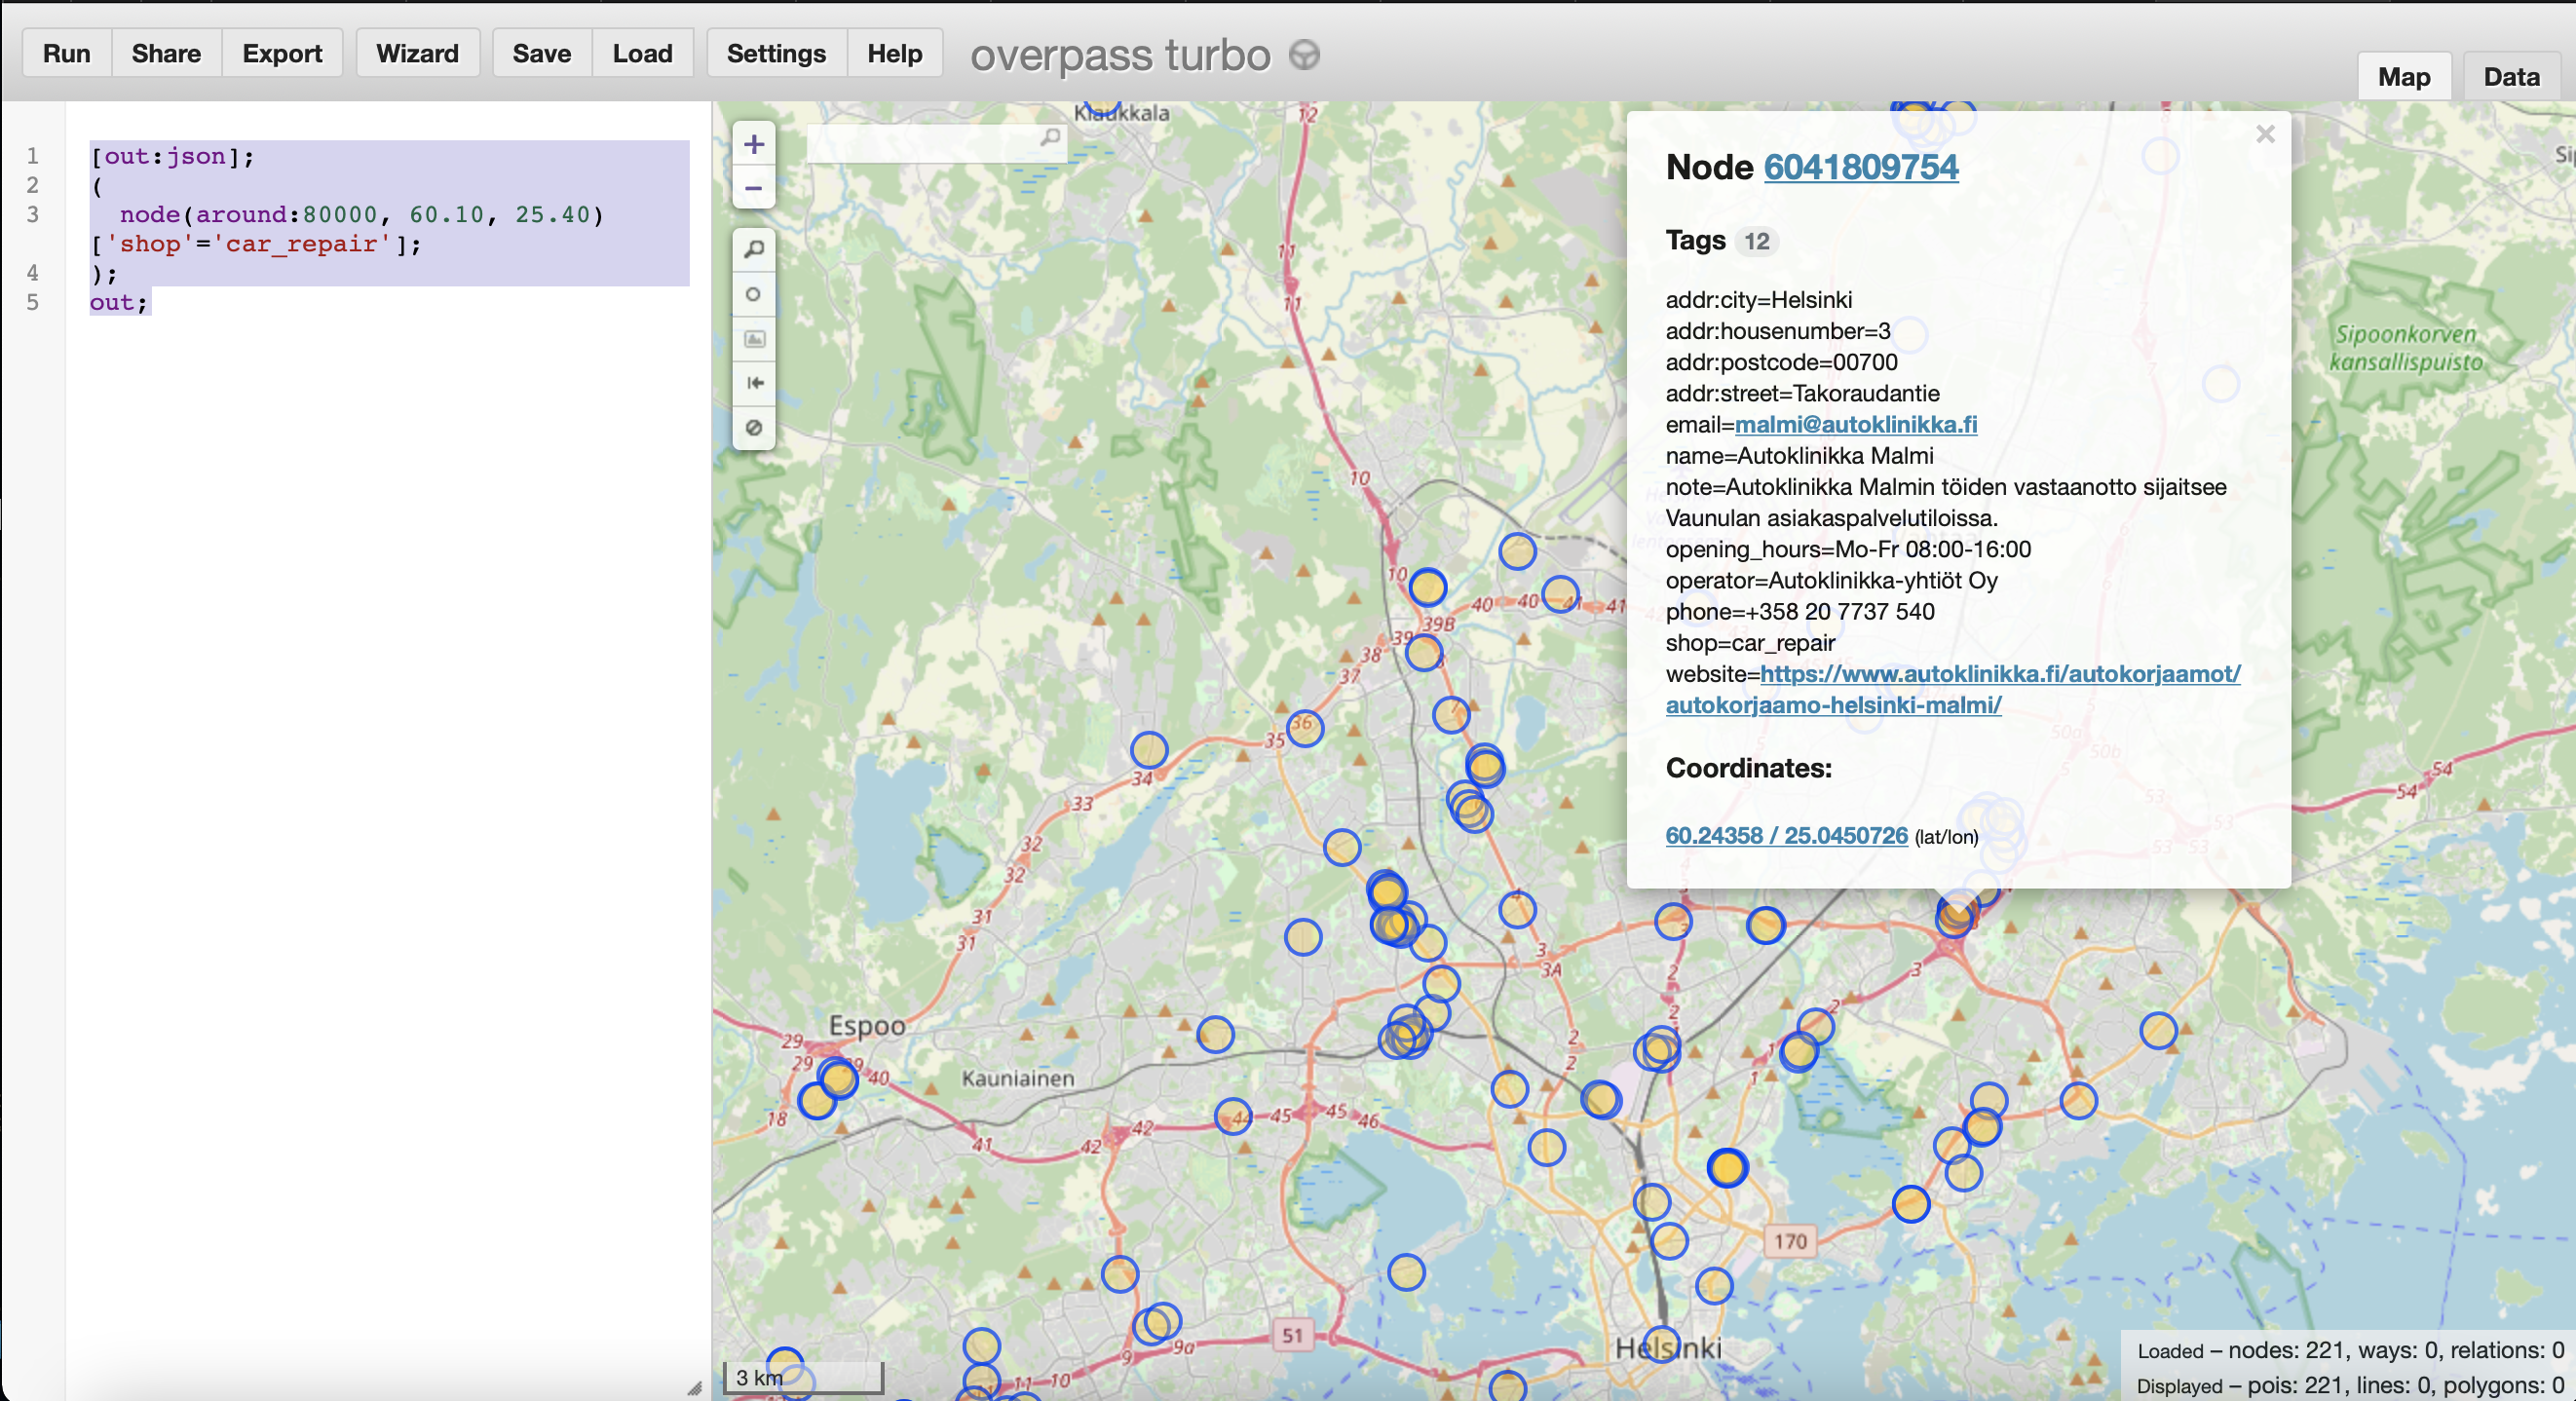
\includegraphics[width=0.9\textwidth]{images/grafici/overpass_primer.png}
    \caption{Open Street Map, Overpass API}
    \label{fig:osm}
\end{figure}
\end{frame}

\begin{frame}{Podaci - vremenske serije}
-- jednostavne vremenske serije (univarijantne)
\vspace{-10px}

\begin{columns}
\begin{column}{0.5\textwidth}
\begin{table}
\centering
\caption{Primer korišćenih podataka za dnevnu vremensku seriju (prvih 7 vrednosti)}
\label{tbl: daily_data_example}
\begin{tabular}{ |c|c|} 
\hline
date & demand\_value \\
\hline
2019-12-18 & 0.098\\
2019-12-19 & 0.245\\
2019-12-20 & 0.402\\
2019-12-23 & 0.490\\
2019-12-27 & 0.520\\
2019-12-28 & 0.020\\
2019-12-30 & 0.500\\
\hline
\end{tabular}
\end{table}
\end{column}

\begin{column}{0.5\textwidth}
\begin{table}
\centering
\caption{Primer korišćenih podataka za nedeljnu vremensku seriju (prvih 7 vrednosti)}
\label{tbl: weekly_data_example}
\begin{tabular}{ |c|c|} 
\hline
year\_week & demand\_value \\
\hline
201951 & 0.144\\
201952 & 0.295\\
202001 & 0.140\\
202002 & 0.333\\
202003 & 0.790\\
202004 & 0.921\\
202005 & 0.915\\
\hline
\end{tabular}
\end{table}
\end{column}
\end{columns}

\end{frame}

\section{Prikaz rezultata}
\begin{frame}{Dnevni nivo}
\begin{itemize}
\item podaci su grupisani na nivou cele države (Švedske);
\item vremenski period: 18.12.2019 - 29.05.2021;
\item izbačene su sve nedelje, nakon čega su ostala 454 dana u podacima.
\end{itemize}
\vspace{-10px}

\begin{figure}[!ht]
  \centering
  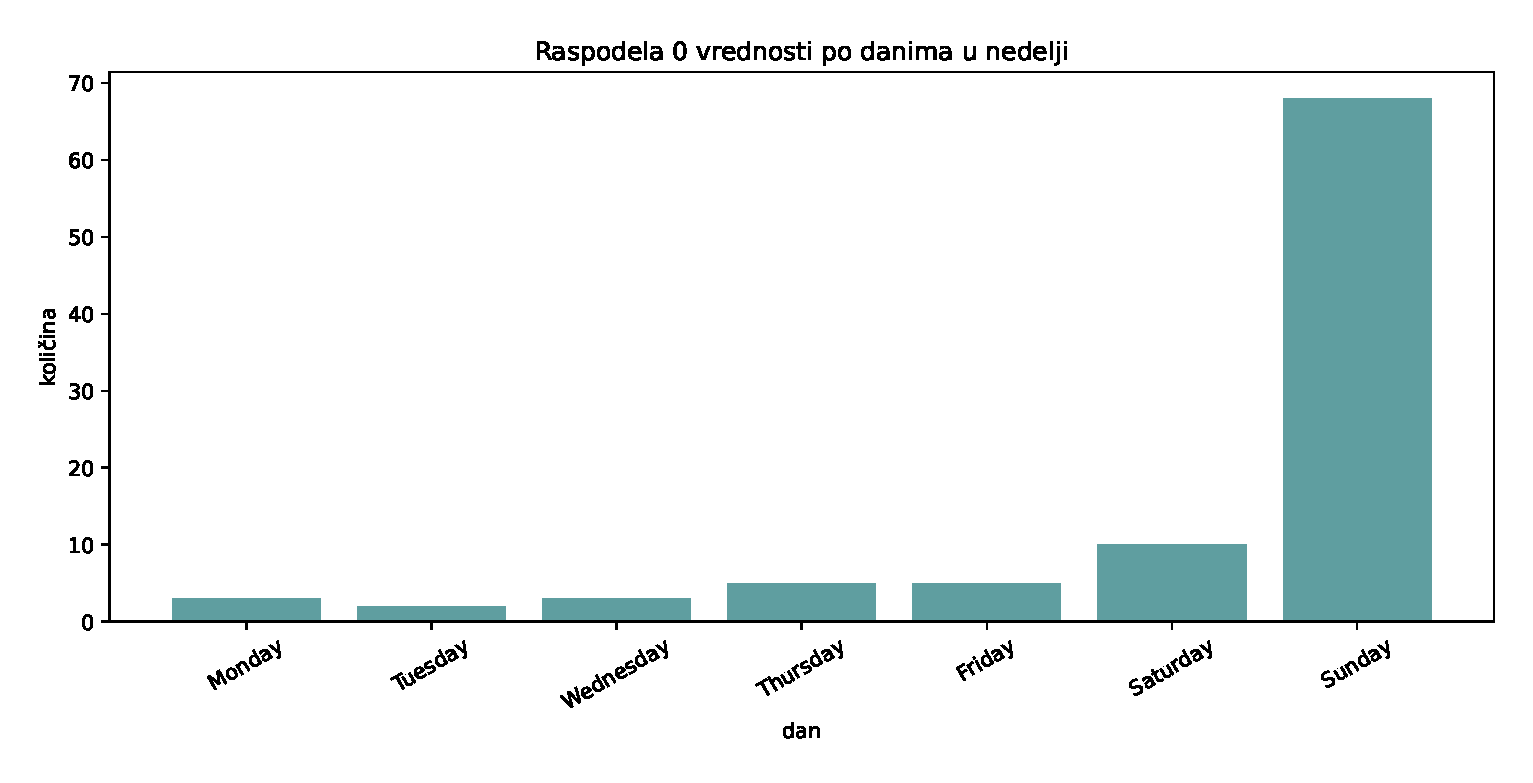
\includegraphics[width=0.75\textwidth]{./images/grafici/nule_po_danima_nedelje.eps}
  \vspace{-10px}
  \caption{Raspodela nula vrednosti promenljive potražnje po danima u nedelji}
  \label{fig: dani_nedelje}
\end{figure}

\end{frame}

\begin{frame}{Dnevni nivo}
    \begin{figure}[!ht]
      \centering
      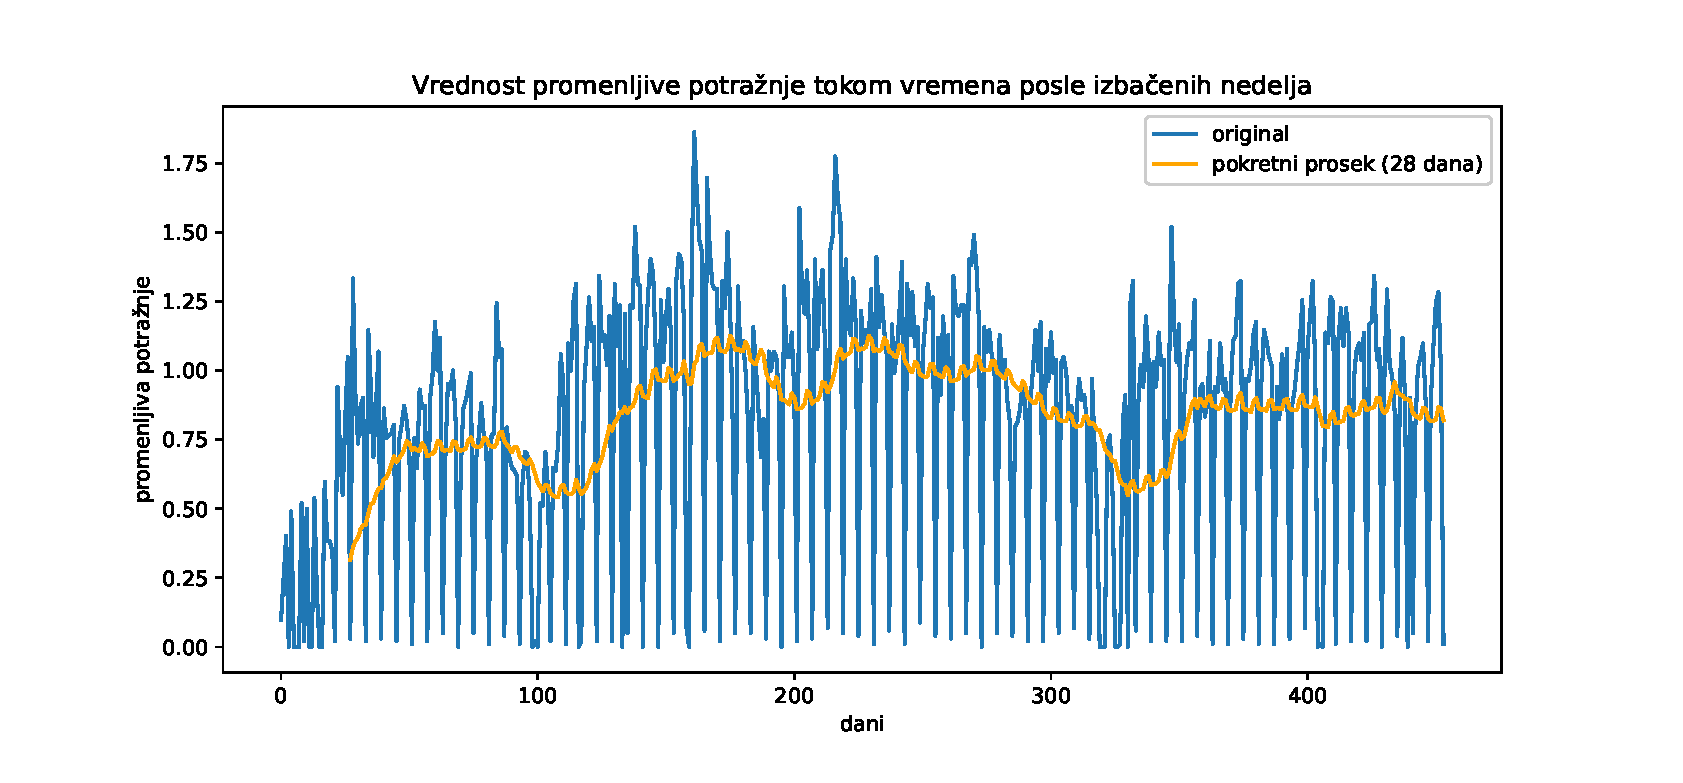
\includegraphics[width=1\textwidth]{./images/grafici/vremenska_serija_primer_bez_nedelja.eps}
      \caption{Vremenska serija bez nedelja}
      \label{fig: dnevna_vremenska_serija_bez_nedelja}
    \end{figure}
\end{frame}

\begin{frame}{Dnevni nivo - ARIMA (stacionarnost, p, q)}
 \begin{figure}[!ht]
    \centering
    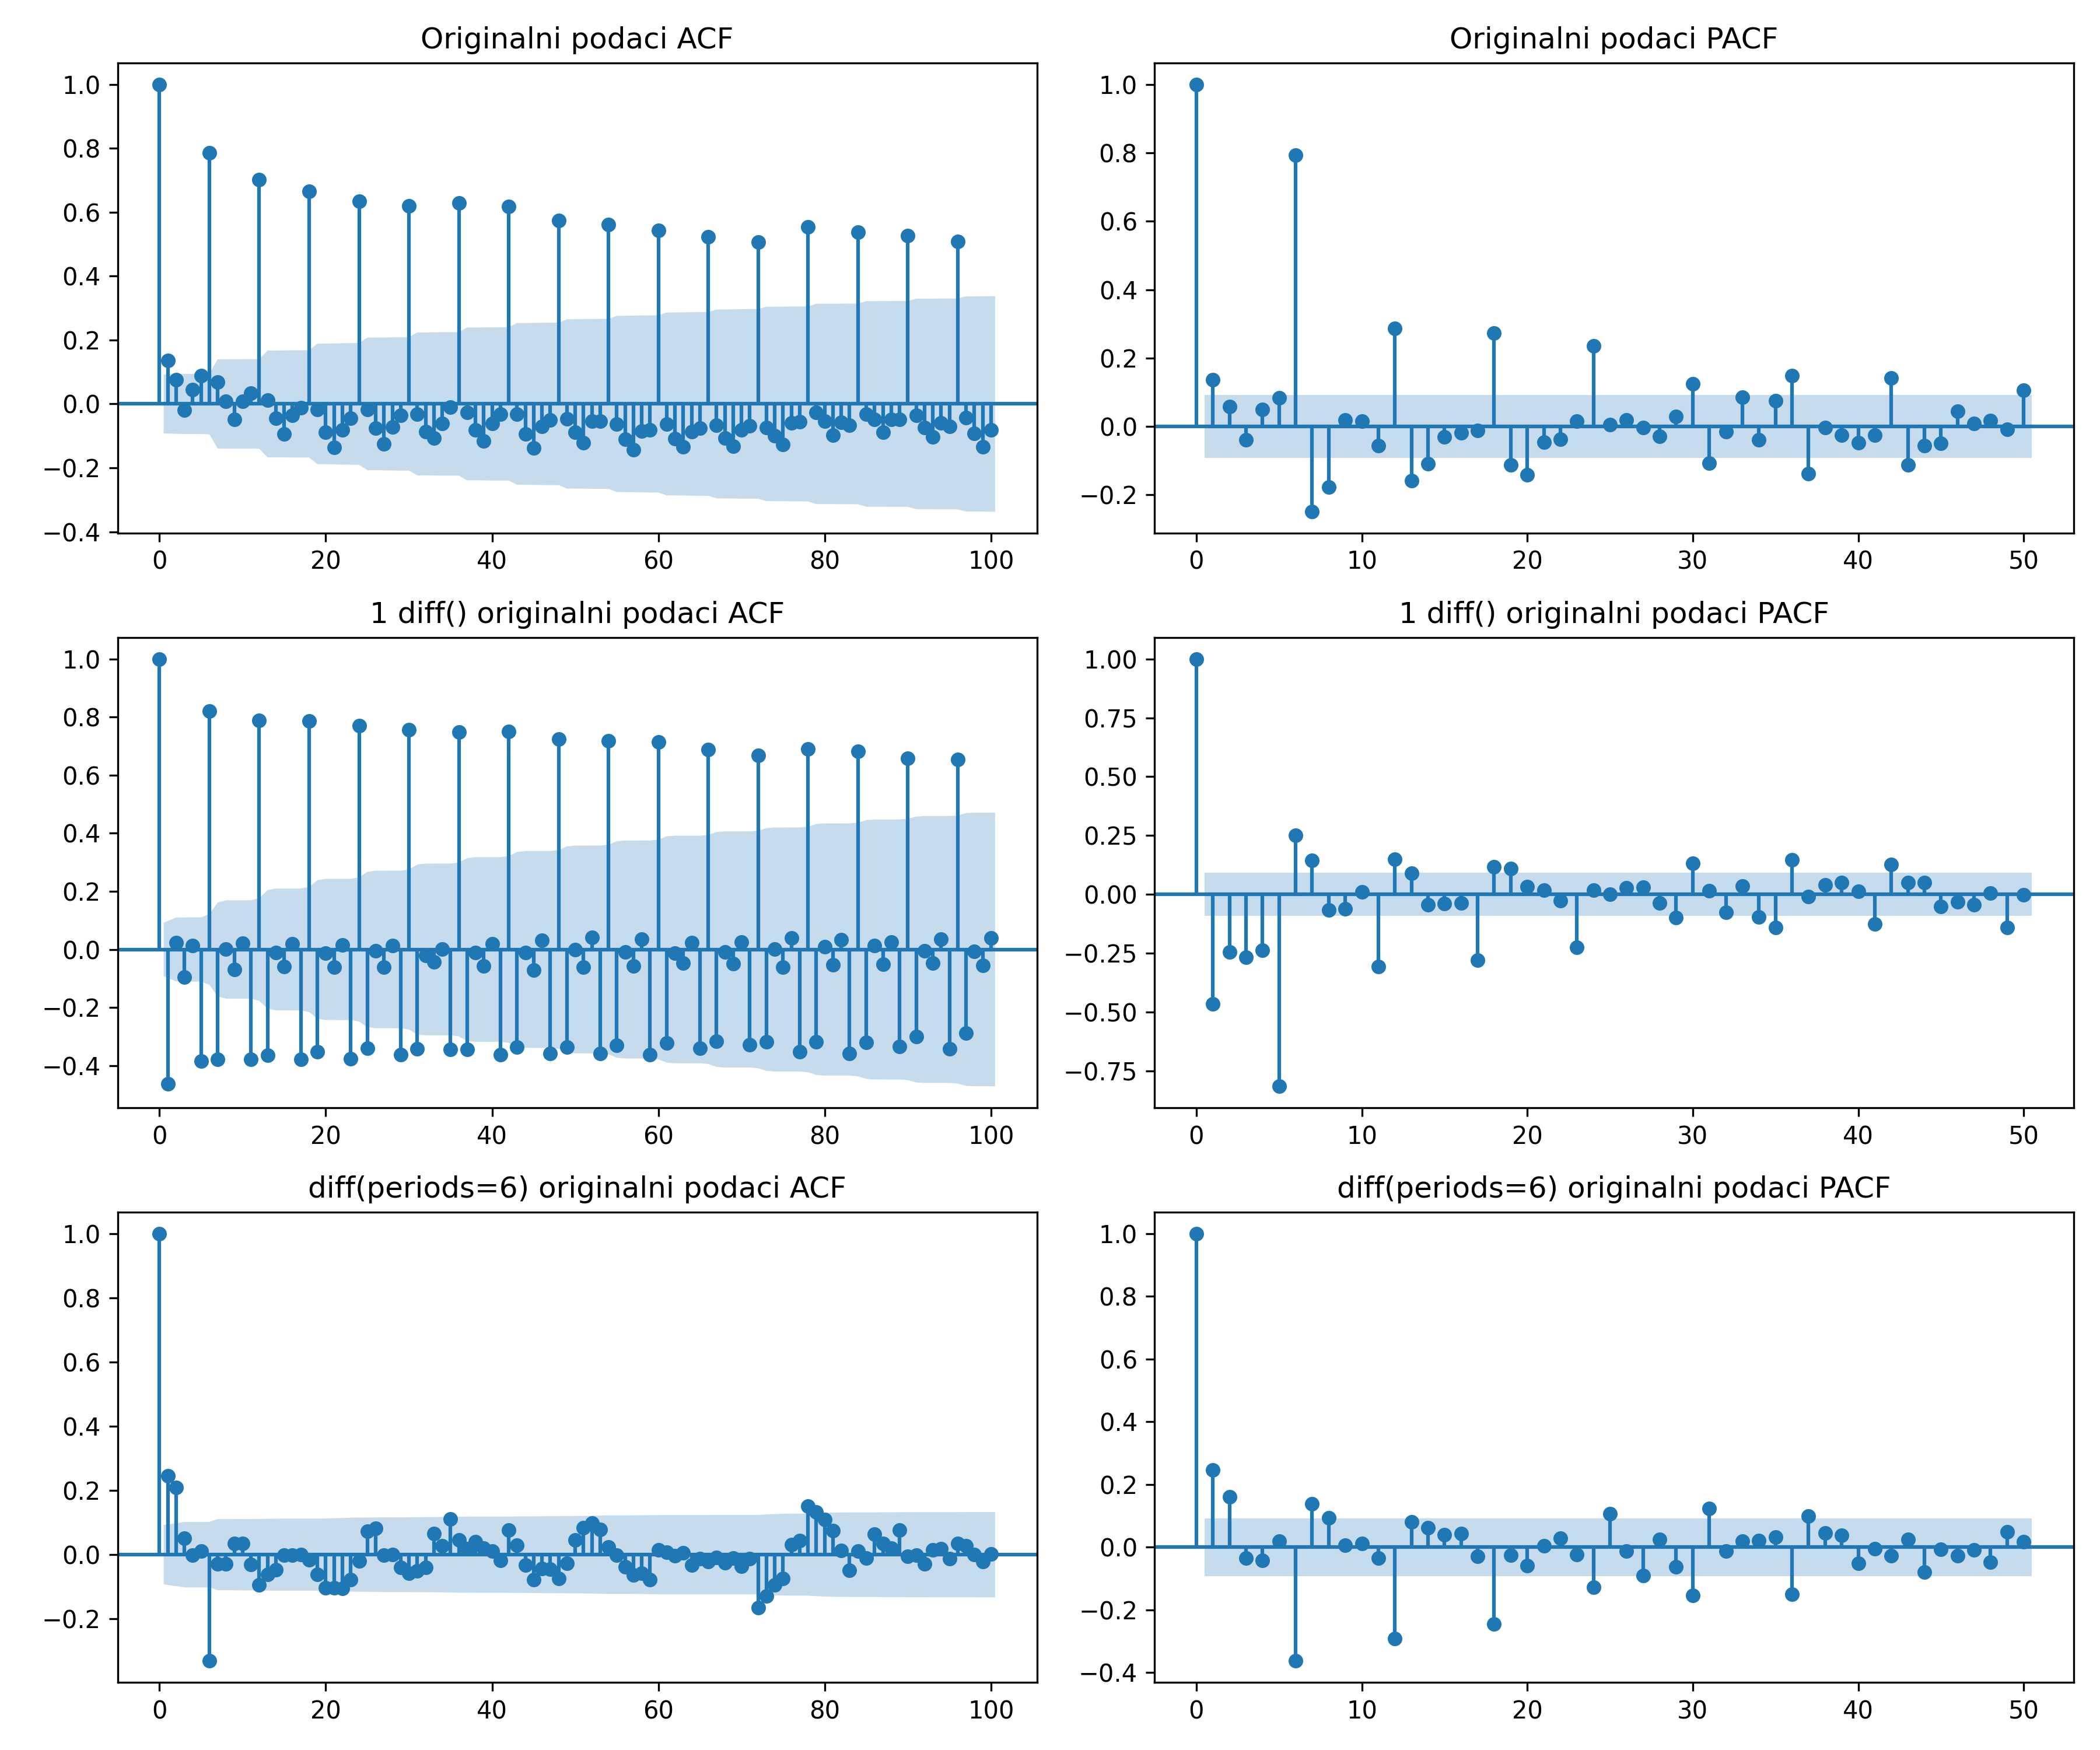
\includegraphics[width=0.6\textwidth]{./images/grafici/acf_pacf_dnevni.png}
    \vspace{-5px}
    \caption{ACF i PACF grafici. Na x-osi su pomeraji, a na y-osi vrednost korelacije}
    \label{fig: acf_pacf_dnevni}
\end{figure}
\end{frame}

\begin{frame}{Dnevni nivo - ARIMA}

\vspace{-7px}
\begin{table}[!ht]
\centering
\caption{SARIMA/ARIMA vrednosti AIC metrike}
\vspace{-3px}
\label{tbl: arime_aic}
\resizebox{0.4\columnwidth}{!}{%
\begin{tabular}{ |l|c| } 
\hline
MODEL & AIC \\
\hline
ARIMA(1, 0, 1) & 567.39\\ 
ARIMA(1, 0, 0) & 598.30\\ 
ARIMA(6, 0, 6) & 14.31\\ 
ARIMA(9, 0, 6) & 14.63\\
ARIMA(1, 0, 1)(1, 0, [1,2])$_6$ & 3.81\\
ARIMA(2, 0, 0)(2, 0, 1)$_6$ & 8.57\\
\hline
\end{tabular}
}
\end{table}

\vspace{-7px}
\begin{table}[!ht]
\centering
\caption{SARIMA/ARIMA metrike evaluacije}
\vspace{-3px}
\label{tbl: arime_metrike}
\resizebox{0.7\columnwidth}{!}{%
\begin{tabular}{ |l|c|c|c|c|} 
\hline
MODEL & MAE & MSE & RMSE & SMAPE \\
\hline
ARIMA(1, 0, 1) & 0.390 & 0.230 & 0.480 & 0.379 \\ 
ARIMA(1, 0, 0) & 0.383 & 0.216 & 0.465 & 0.376\\ 
ARIMA(6, 0, 6) & 0.564 & 0.094 & 0.307 & 0.213\\ 
ARIMA(9, 0, 6) & 0.209 & 0.095 & 0.309 & 0.224\\ 
ARIMA(1, 0, 1)(1, 0, [1,2])$_6$ & 0.192 & 0.095 & 0.308 & 0.208\\
ARIMA(2, 0, 0)(2, 0, 1)$_6$ & 0.200 & 0.092 & 0.304 & 0.216\\
\hline
\end{tabular}
}
\end{table}
\end{frame}

\begin{frame}{Dnevni nivo - ARIMA}
\begin{itemize}
    \item Trening skup: svi dani pre 01.03.2021.
    \item Predviđanje 1 po 1 dan u budućnost
\end{itemize}

\begin{figure}[!ht]
  \centering
  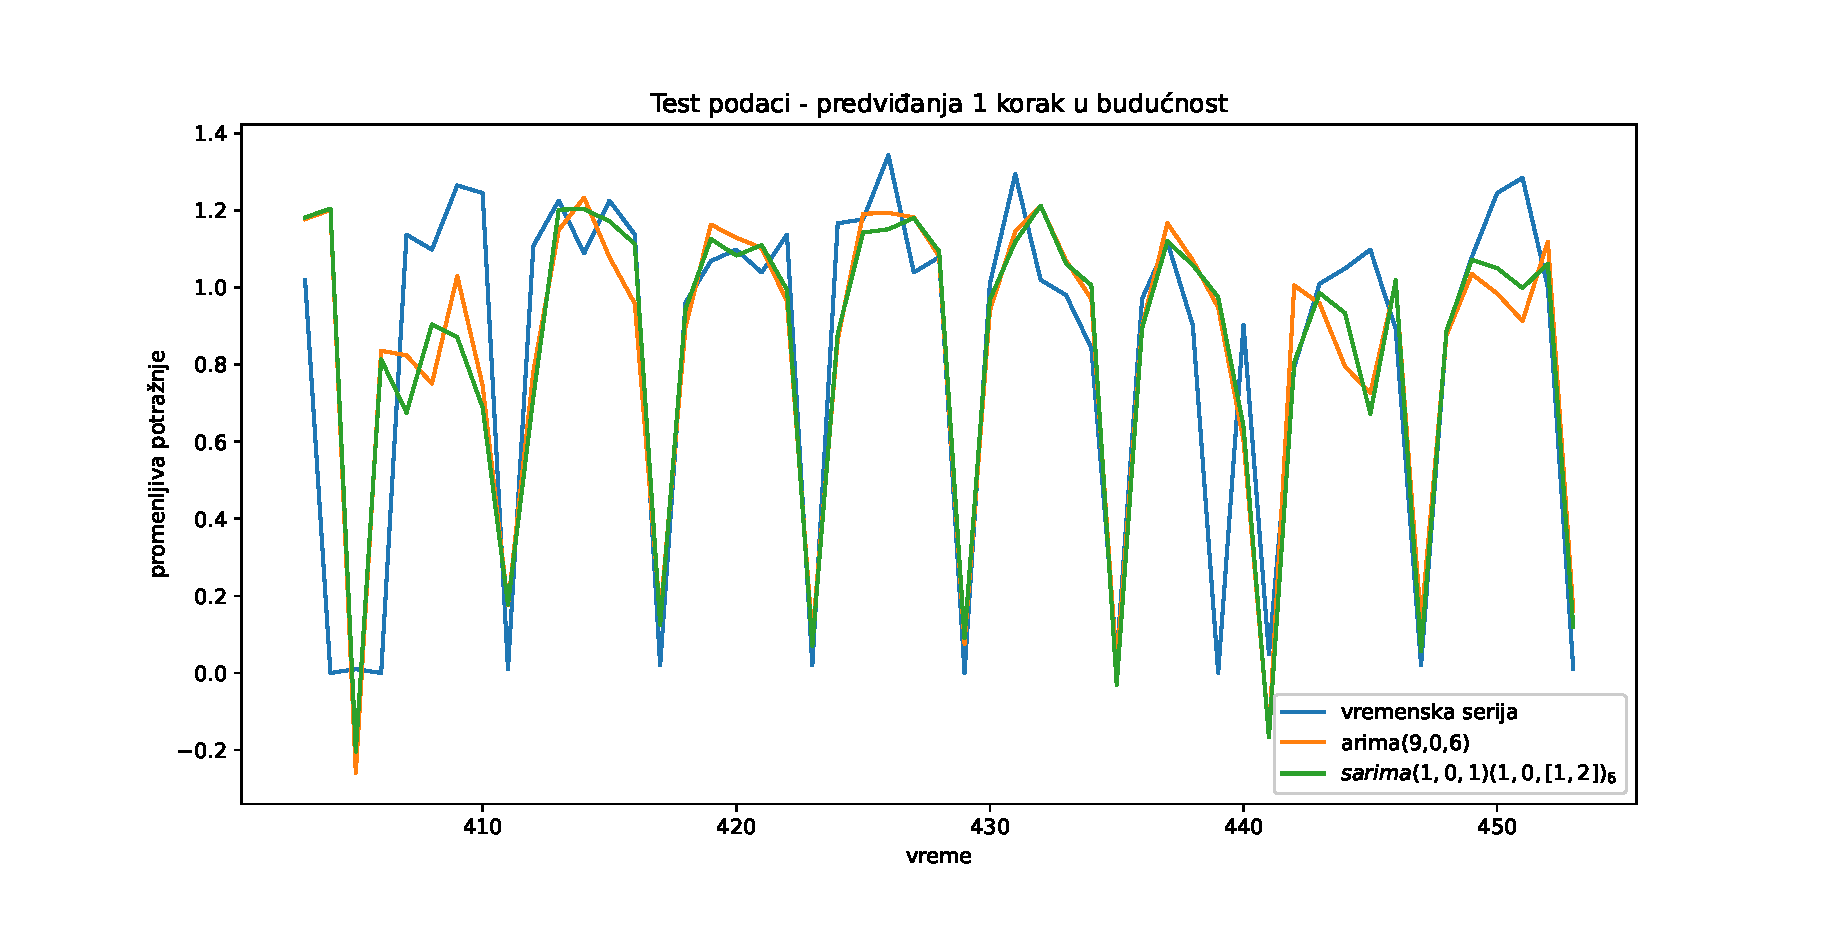
\includegraphics[width=1\textwidth]{./images/grafici/test_dnevna_arima.eps}
  \caption{Ponašanje jedan po jedan korak predviđanja dva modela kod ARIMA metode}
  \label{fig: test_arima}
\end{figure}

\end{frame}

\begin{frame}{Dnevni nivo - Prophet}
\begin{itemize}
    \item Uračunavanje praznika u model
\end{itemize}    
\vspace{-8px}
\begin{table}
\centering
\caption{Prophet metrike evaluacije}
\vspace{-8px}
\label{tbl: prophet_dnevni}
\resizebox{0.6\columnwidth}{!}{%
\begin{tabular}{ |l|c|c|c|c|} 
\hline
MODEL & MAE & MSE & RMSE & SMAPE \\
\hline
prophet (w, m, h) & 0.121 & 0.038 & 0.196 & 0.141 \\ 
prophet (w, m, h, flexible) & 0.113 & 0.032 & 0.180 & 0.130\\
prophet (d, w, m, h) & 0.119 & 0.035 & 0.188 & 0.139 \\
prophet (d, w, m, h, flexible) & 0.114 & 0.032 & 0.180 & 0.130\\
\hline
\end{tabular}
}
\end{table}
\vspace{-12px}
\begin{figure}[!ht]
  \centering
  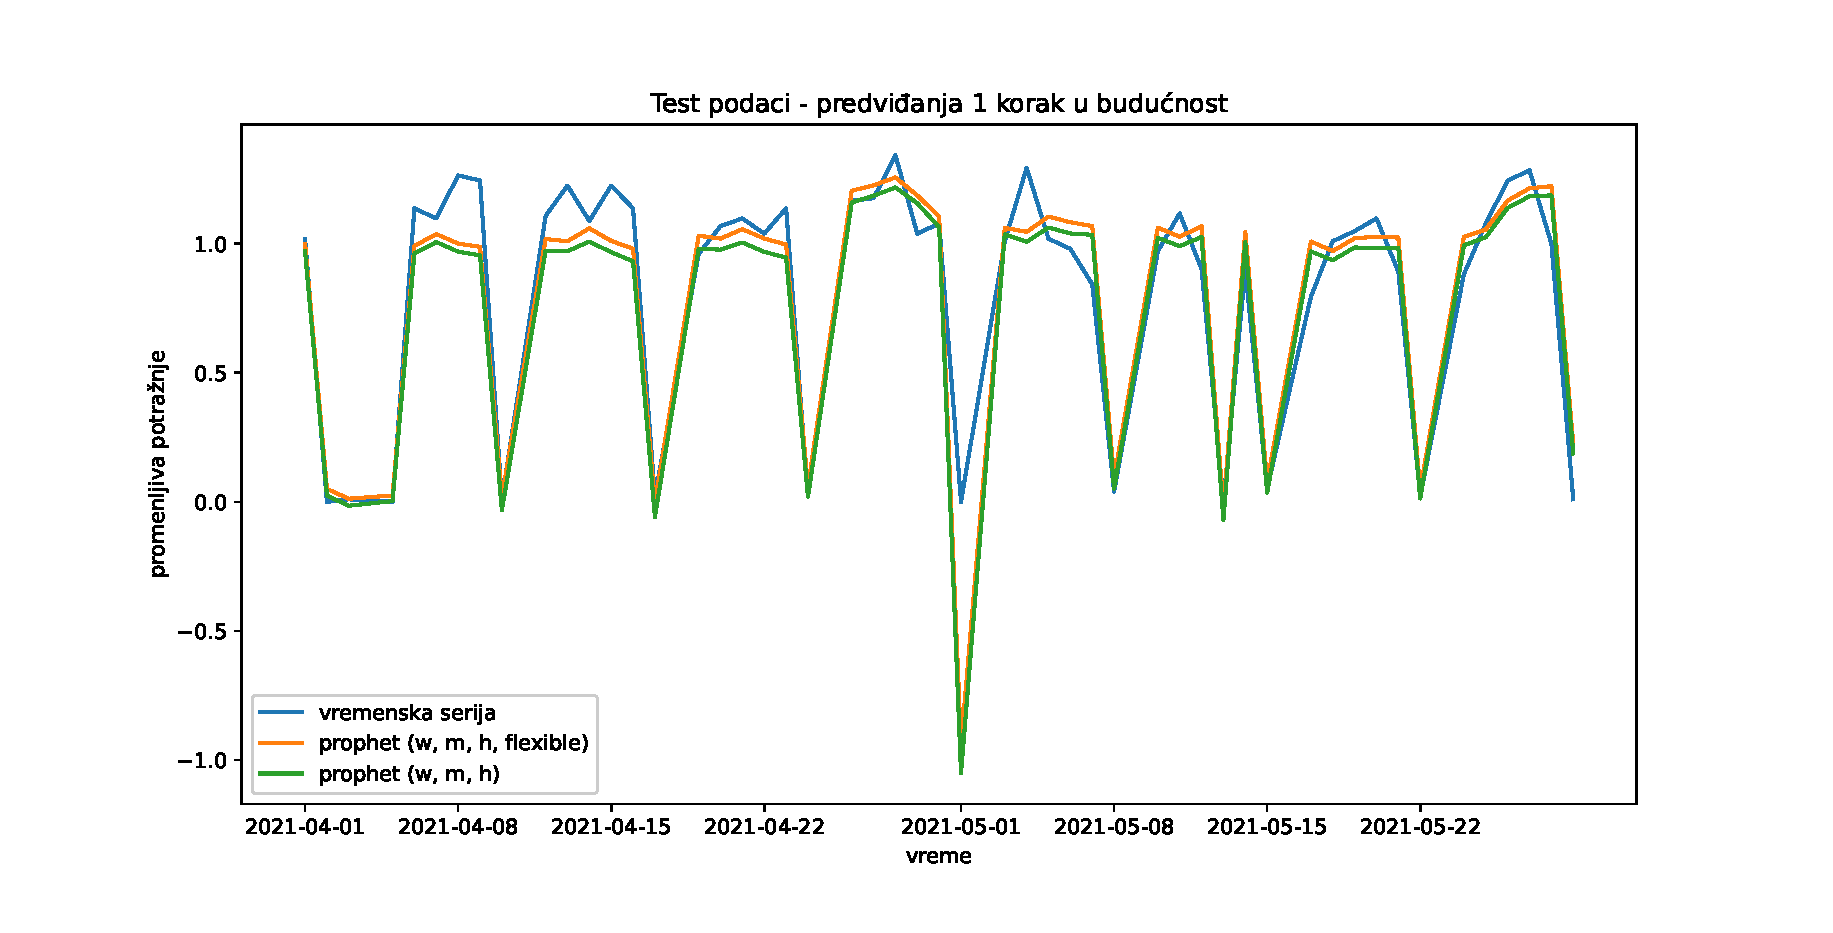
\includegraphics[width=0.8\textwidth]{./images/grafici/test_dnevni_prophet.eps}
  \caption{Ponašanje jedan po jedan korak predviđanja dva modela kod Prophet metode}
  \label{fig: test_prophet}
\end{figure}

\end{frame}

\begin{frame}{Dnevni nivo - XGBoost}
\begin{itemize}
    \item \footnotesize{Atributi su vrednosti promenljive potražnje iz prethodnih nekoliko dana}
    \item \footnotesize{30 vrednosti iz prošlosti + 3 atributa za praznike}
\end{itemize}

\begin{figure}[!ht]
  \centering
  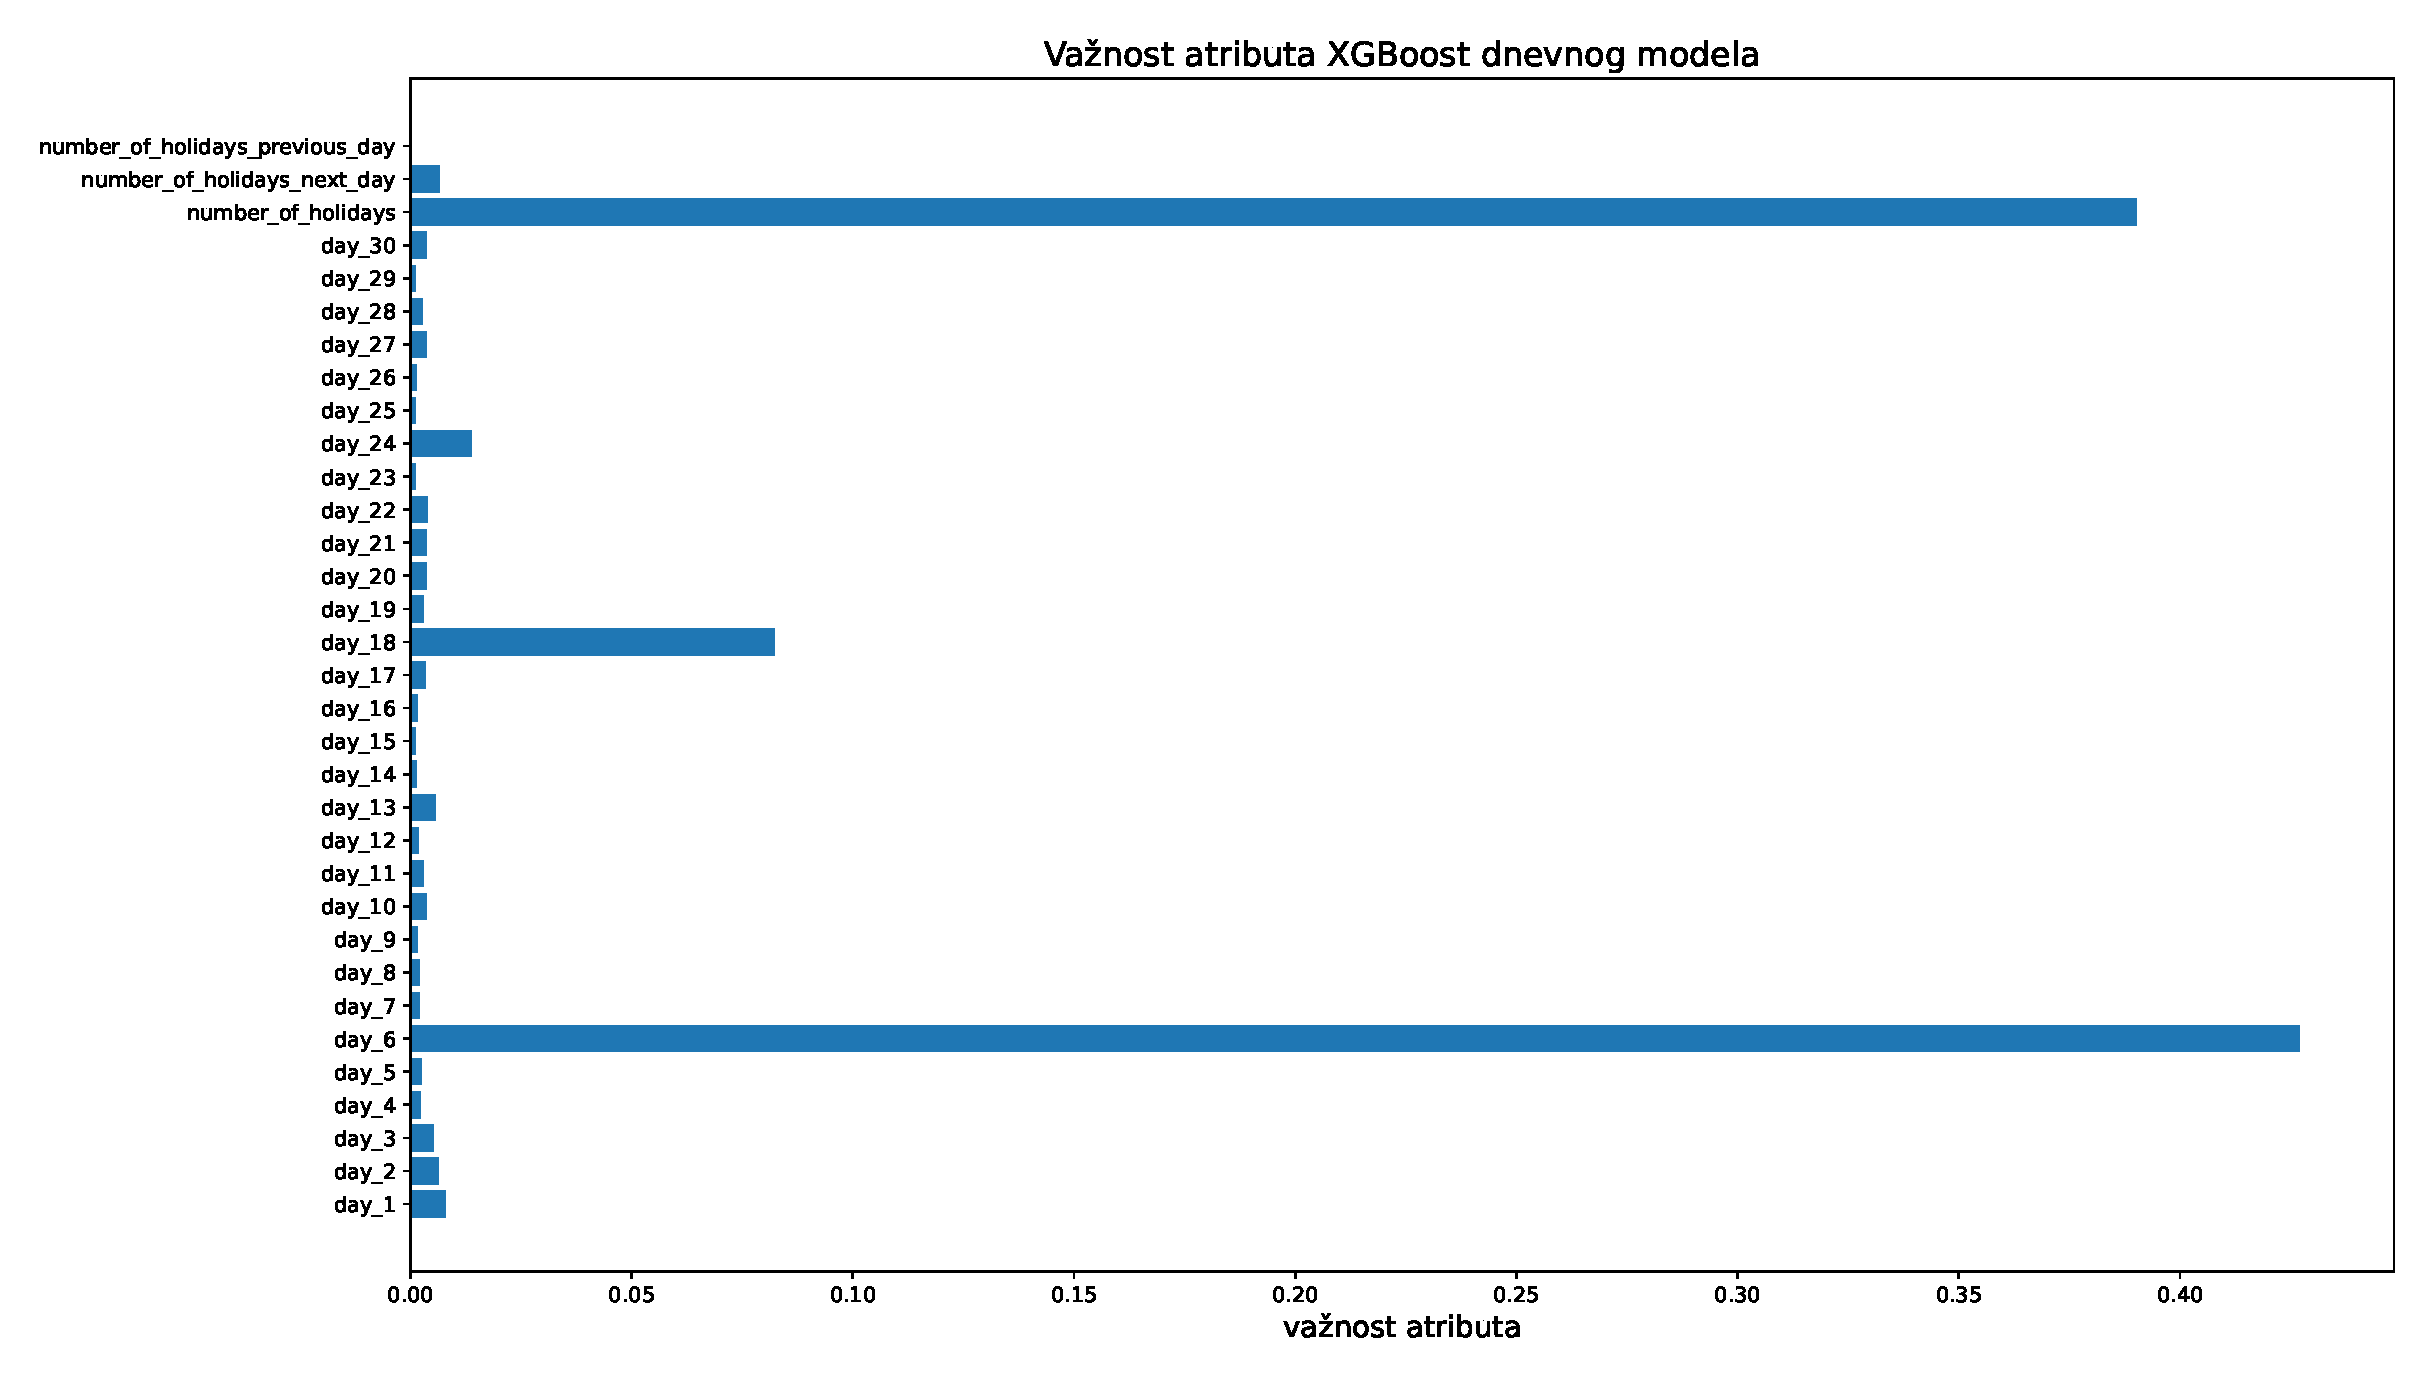
\includegraphics[width=0.83\textwidth]{./images/grafici/vaznost_atributa.eps}
  \vspace{-6px}
  \caption{\footnotesize{Važnost atributa kod XGBoost dnevnog modela}}
  \label{fig: vaznost_atributa}
\end{figure}

\end{frame}


\begin{frame}{Nedeljni nivo}
\begin{itemize}
    \item \footnotesize {76 dostupnih nedelja;}
\end{itemize}

\begin{table}
\centering
\caption{Evaluacione metrike nad test podacima nedeljne vremenske serije}
\label{tbl: nedeljna_serija_metrike}
\resizebox{0.7\columnwidth}{!}{%
\begin{tabular}{ |l|c|c|c|c|} 
\hline
MODEL & MAE & MSE & RMSE & SMAPE\\
\hline
prophet (w, m, h) & 0.180 & 0.052 & 0.227 & 0.164\\
prophet (w, m, h, flexible) & 0.145 & 0.038 & 0.195 & 0.144\\
ARIMA(1, 0, 0) & 0.155 & 0.041 & 0.203 & 0.151\\
ARIMA(1, 1, 1) & 0.162 & 0.046 & 0.216 & 0.155\\
ARIMA(1, 0, 2) & 0.159 & 0.042 & 0.205 & 0.154\\
ARIMA(12, 1 ,0) & 0.163 & 0.046 & 0.215 & 0.157\\
ARIMA(13, 0, 2) & 0.162 & 0.044 & 0.210 & 0.158\\
\hline
\end{tabular}
}
\end{table}

\begin{table}
\centering
\caption{Metrike evaluacije nad test podacima nedeljnog XGBoost modela}
\label{tbl: xgboost_nedeljni_metrike}
\resizebox{0.4\columnwidth}{!}{%
\begin{tabular}{ |l|c|c|c|} 
\hline
MAE & MSE & RMSE & SMAPE\\
\hline
0.146 & 0.046 & 0.215 & 0.139\\
\hline
\end{tabular}
}
\end{table}
    
\end{frame}

\begin{frame}{XGBoost - veća granularnost}
\begin{itemize}
    \item  Sitniji nivo predviđanja: nivo automehaničarskih radnji i marki automobila;
    \item Isprobana su 4 modela;
\end{itemize}

\begin{table}
\centering
\caption{XGBoost metrike evaluacije za 4 modela}
\label{tbl: xgboost_atributi}
\resizebox{0.7\columnwidth}{!}{%
\begin{tabular}{ |l|c|c|c|c|} 
\hline
MODEL & MAE & MSE & RMSE & SMAPE \\
\hline
year\_week\_garage\_category & 0.3044& 0.257 & 0.507 & 0.315 \\ 
year\_month\_garage\_make & 0.175 & 0.112 & 0.334 & 0.201 \\
year\_week\_garage\_make & 0.183 & 0.129 & 0.359 & 0.207 \\
year\_month\_garage\_category & 0.331 & 0.278 & 0.528 & 0.316 \\
\hline
\end{tabular}
}
\end{table}
\end{frame}

\begin{frame}{XGBoost - veća granularnost}

\begin{figure}[!ht]
  \centering
  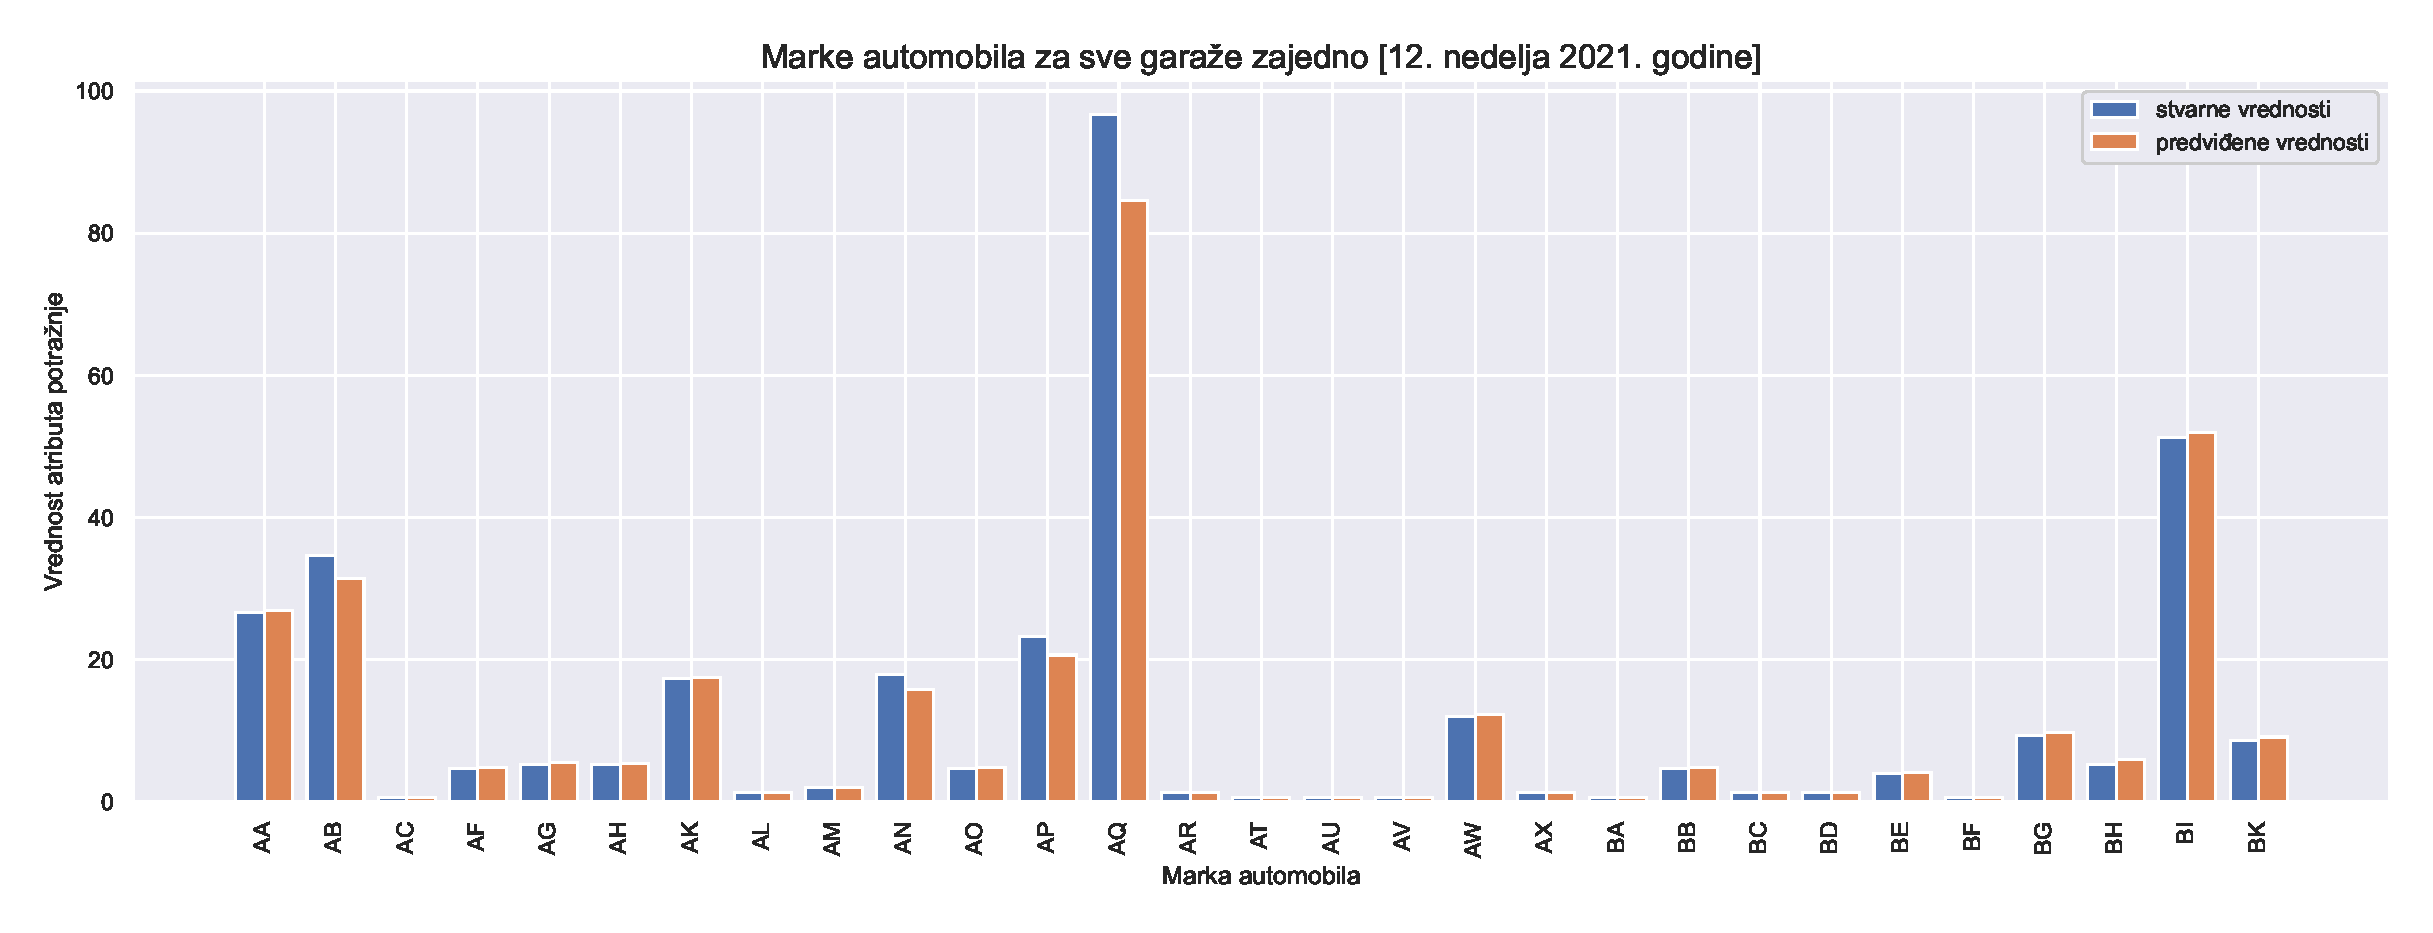
\includegraphics[width=0.75\textwidth]{./images/grafici/year_week_garage_make_train_on_all_available_202112.eps}
  \vspace{-10px}
  \caption{\footnotesize{Raspodela marki automobila za 12. nedelju 2021. godine}}
  \label{fig: marke_nedelja}
\end{figure}
\vspace{-17px}
\begin{figure}[!ht]
  \centering
  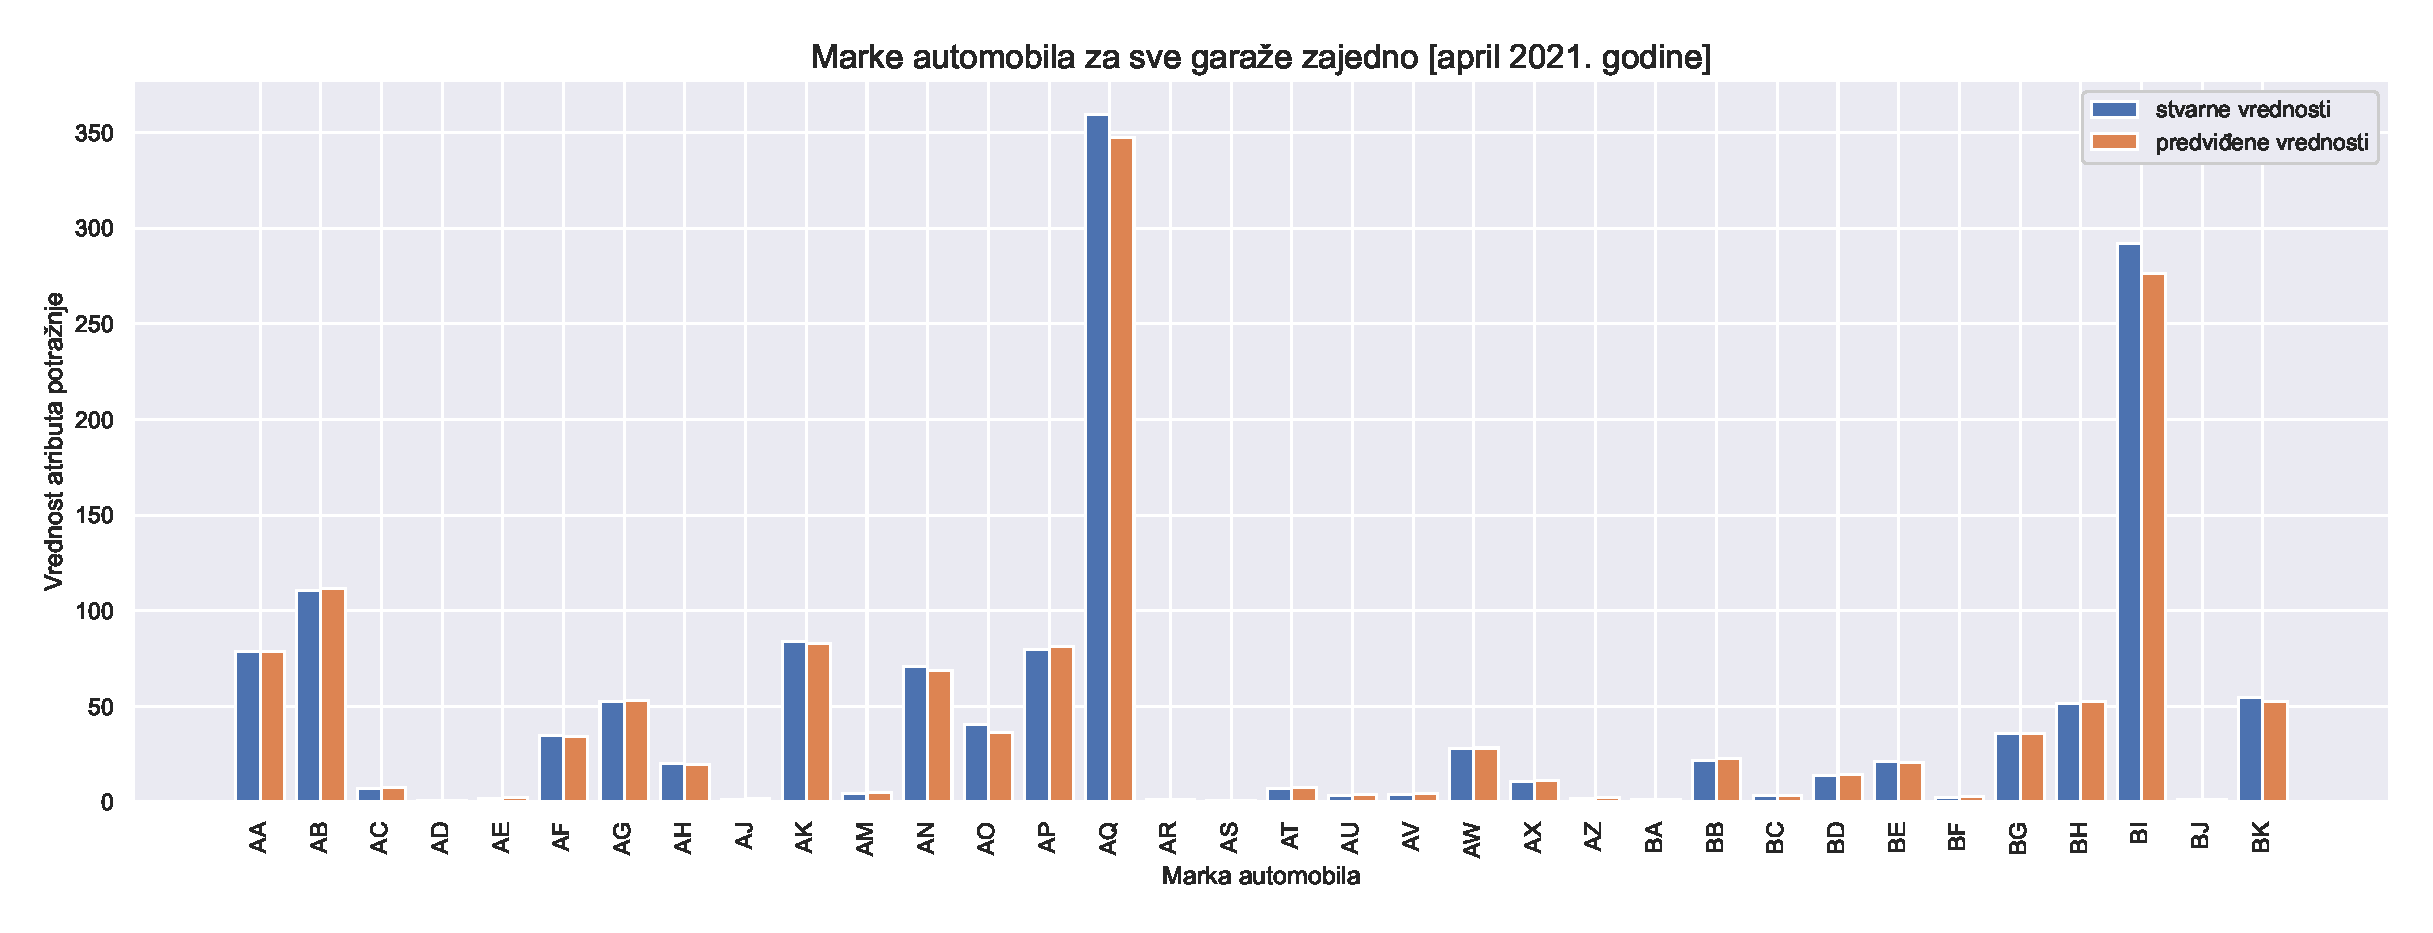
\includegraphics[width=0.75\textwidth]{./images/grafici/year_month_garage_make_train_on_all_available_202104.eps}
  \vspace{-10px}
  \caption{\footnotesize{Raspodela marki automobila za april mesec 2021. godine}}
  \label{fig: marke_mesec}
\end{figure}

\end{frame}

\section{Diskusija i zaključak}
\begin{frame}{Diskusija i zaključak}
\begin{itemize}
    \item Nedovoljna količina podataka; 
    \item Potencijalno nestandardni podaci: pandemija Kovid19 virusa;
    \item Problem sa malim radnjama;
    \item Kombinovanje zaključaka dobijenih ARIMA metodom sa XGBoost metodom;
    \item Obogaćivanje eksternim podacima (vremenska prognoza, procenjena cena automobila);
    \item Klasifikacija + regresija?
\end{itemize}
\end{frame}

\section{Pitanja}
\begin{frame}
Hvala na pažnji.
\newline
\vspace{30pt}Pitanja?
\end{frame}

% \section{Literatura}
% \begingroup
% \setbeamertemplate{footline}{}
% \begin{frame}{Literatura}
% \scalebox{0.83}
% {
% \begin{minipage}{1.20\textwidth}
% \bibliography{literatura} 
% \bibliographystyle{plain}
% % \nocite{wagner1997practical}
% \end{minipage}
% }
% \end{frame}
% \endgroup


\setbeamertemplate{footline}{\hspace*{.5cm}\scriptsize{\hspace*{50pt} \hfill\hspace*{.5cm} \setbeamercolor{black}}\\
\vspace{9pt}}

\setbeamertemplate{headline}{\hspace*{.5cm}\scriptsize{\hspace*{50pt} \hfill\hspace*{.5cm} \setbeamercolor{black}}\\
\vspace{1pt}}

% \setbeamercolor{mysection in head/foot}{bg= black,fg=black}
\end{document}